%! TEX root = ../thesis.tex

\chapter{Physics of cosmic rays}
\label{chap:physical-background}

This chapter aims to introduce the general physical principles underlaying the analysis presented in this work. For this purpose, an overview of the origin, 
composition and energy spectrum of cosmic rays is given in \autoref{ssec:cr-history}, \autoref{sec:cr-origin}, and \autoref{sec:cr-energy-spectrum} respectively. 
Their interactions with other matter, the physics of extensive air showers and their possible detection methods are listed in \autoref{sec:extensive-air-showers}.

\section{History}
\label{ssec:cr-history}

A first hint at the existance of high-energy particles in the upper atmosphere was given by Hess in 1912, who found that the discharge rate of an electroscope is 
altitude-dependant. Millikan coined the term cosmic "rays" for these particles, as he argued the ionizing radiation must be part of the electromagnetic spectrum 
\cite{millikan1928origin}. This was later, at least partially, falsified with the discovery of the east-west effect \cite{johnson1938note}. Hess' observation 
however withstood the tests of time and was ultimately recognized with the Nobel prize in physics in 1936 \cite{nobelprize1936}. Two years later, in 1938, Pierre 
Auger showed via coincidence measurements that cosmic rays in fact originate from outer space, and gave a first description of extensive air showers 
\cite{auger1939extensive}. Another 60 years later, the Pierre Auger collaboration would adopt his experimental setup and name in their search for cosmic rays of 
the highest energies.

In the meantime, numerous results from different cosmic ray detectors all over the globe have helped propel the related fields of particle physics, astro physics 
and cosmology to new insights. Observations from cosmic ray physics serve as a valuable cross-check to the hadronic interaction models developed e.g. at CERN 
\cite{ostapchenko2007status}. New theories modeling the final moments in the life of stars have arisen thanks to results from e.g. Kamiokande 
\cite{goldman1988implications}. Last but not least publications by the Pierre Auger collaboration regarding the CR energy spectrum and flux help refine knowledge of 
our cosmic neighbourhood \cite{abraham2010measurement, aab2015searches}.

\section{Origin}
\label{sec:cr-origin}

\subsection{Acceleration}
\label{ssec:cr-acceleration}

Cosmic rays whose kinetic energy far exceeds their rest energy must originate from some of the most extreme environments in space. In particular, regions with 
large (either in field strength or spatial extent) electromagnetic fields, where charged particles can be accelerated to significant fractions of to the speed of 
light, via the Lorentz force. 

The question how particles are accelerated to the extremely high energies observed on earth is an active area of research. Since the discovery of cosmic rays, 
several candidate mechanisms and interactions have been identified and will be discussed now.

\subsubsection{Diffusive shock acceleration (Fermi I)}
\label{sssec:cr-fermi-i}

\textbf{S}uper \textbf{N}ova \textbf{R}emnants (SNR) typically feature a plasma sphere propagating outwards from the former stars core into the 
\textbf{I}nter \textbf{S}tellar \textbf{M}edium (ISM), in this region of plasma any magnetic field lines will be comoving, according to Alfvén's theorem 
\cite{alfven1942existence}. First realised by Fermi, such SNR shock fronts serve as source of high-energy CRs \cite{fermi1949origin}.

If a low-energy particle is injected into the SNR shock front, it will eventually be reflected by the local $\vec{B}$-field. If the diffusion length within the
plasma is much smaller than the spatial extent of the SNR, the shock front can be modelled as a plane, and the process is analogous to an elastic reflection 
against a wall. Consequently, if $\frac{\text{d}\vec{B}}{\text{d}t} = 0$, this does not cause the particle to gain any energy, espically because 
$W = \vec{F}_\text{L} \cdot \vec{r} \propto (\vec{v}\times\vec{B})\,\cdot\,\vec{r} = 0$. However, because the $\vec{B}$-field is moving radially outward alongside 
the plasma, a net energy gain of 

\begin{equation}
\label{eq:fermi-energy-gain}
\Delta E = +\beta_\text{SNR} \cdot E_0
\end{equation}

arises, where $\beta_\text{SNR} = |\vec{v}_\text{SNR}|\,/\,c$ and $E_0$ are the velocity of the shock-front and the initial energy of the particle. From chapter 7 
in \cite{fermi1949origin} it follows that ionization losses within the shock front are not completely negligible. Hence a particle must have a sufficient energy 
such that $\Delta E$ in \autoref{eq:fermi-energy-gain} exceeds possible ionization losses. The corresponding threshold for the primary energy above which 
acceleration occurs is dubbed the injection energy, and is of the order of \SI{200}{\mega\electronvolt} for protons. 

Furthermore, because typically $\beta_\text{SNR} \leq 0.10$ a single acceleration cycle is not enough to explain the CR energies observed on earth. Instead, 
multiple cycles are needed. This requires additional, focusing $\vec{B}$-fields, provided for example by the ISM, which alter the trajectory of injected particles 
such that they can be reflected off the shock-front again.

With each cycle, the particles rigidity $R = |\vec{p}|c\,/\,q$ increases, until its gyroradius $\rho = R / |\vec{B}|$ exceeds the spatial extent of the focusing 
$\vec{B}$-field and the particle escapes into space. With an effective ejection probability $p$ per cycle, the energy after $n$ cycles and the expected flux w.r.t
energy, $\Upphi(E)$, becomes roughly

\begin{equation}
\label{eq:fermi-energy}
E(n) = E_0\;\left( 1 + \beta_\text{SNR} \right)^n.
\end{equation}

\begin{align*}
                                                        N(n) &= N_0 \;\left( 1 - p \right)^n \\
\Leftrightarrow\;\;\;\;\,\log\left( \frac{N(n)}{N_0} \right) &= n\cdot\log\left( 1-p \right) \\ 
\Leftrightarrow\qquad\qquad\qquad\;\;&\stackrel{\mathmakebox[\widthof{=}]{\eqref{eq:fermi-energy}}}{=}\;\log\left( \frac{E(n)}{E_0} \right) 
\frac{\log(1-p)}{\log(1+\beta_\text{SNR})} \\
\Leftrightarrow\qquad\qquad                             N(E) &= N_0\cdot\left( \frac{E(n)}{E_0} \right)^{\log(1 - p)\;/\;\log(1 + \beta_\text{SNR})} \\
\Rightarrow \qquad\qquad                           \Upphi(E) &= \frac{ \text{d}N }{ \text{d}E } \propto E(n)^{\alpha - 1}, \numberthis\label{eq:fermi-spectrum}
\end{align*}

where $\alpha = \frac{\log(1 - p)}{\log(1 + \beta_\text{SNR})}$ in \autoref{eq:fermi-spectrum} is a spectral coefficient whose exact value will depend on the age 
of the SNR ($\beta_\text{SNR}$ decreases with age), the injected particle (different primaries have different injection energies and ejection probabilities), as 
well as many other factors that are often not known a priori. It can be observed that the expected spectrum is a power law in the ranges from injection energy to a
cutoff at the highest energies, which arises due to the finite lifetime of SNRs.

Results from several studies (e.g. \cite{aab2015searches, hillas2005can, blasi2013origin}) hint that the presented first order Fermi acceleration mechanism is the 
main source of galactic CRs, extrasolar particles that originate from within the milky way, with energies ranging up to orders 
$\mathcal{O}(\SI{}{\tera\electronvolt})$.

\subsubsection{Stochastic scattering acceleration (Fermi II)}
\label{sssec:cr-fermi-ii}

Second order (or Stochastic) Fermi acceleration is the more general case of \autoref{sssec:cr-fermi-i} and represents the original idea developed by Fermi in 
\cite{fermi1949origin}. The underlaying principle of scattering particles off plasma clouds remains unchanged. However, if the diffusion length within the cloud 
exceeds its radius of curvature, the energy gain per collision instead becomes

\begin{equation}
\Delta E \propto + \left( \beta_\text{SNR}\right)^2 \cdot E_0.
\end{equation}

Logically, this represents a much more inefficient acceleration mechanism, but is nevertheless observed in nature under certain circumstances (c.f. 
\cite{asano2015most}).

\subsubsection{Centrifugal acceleration in rotating $\vec{B}$-fields}
\label{sssec:cr-centrifugal-acceleration}

Some astrophysical objects such as pulsars or \textbf{A}ctive \textbf{G}alactic \textbf{N}uclei (AGNs) possess strong magnetic fields ranging from \SI{1}{\tesla}
for some AGNs \cite{daly2019black} to $\approx\SI{10}{\giga\tesla}$ for magnetars, a subset of pulsars with extremely high magnetic flux densities 
\cite{flowers1977evolution}.

If such objects rotate at an angular velocity $\Omega$, which is in general nonzero, charged particles at a radial distance $r$ from the rotation axis will undergo
centrifugal acceleration. In particular, their Lorentz factor $\gamma$ behaves like \autoref{eq:lorentz-factor-acceleration} \cite{rieger1999particle}.

\begin{equation}
\label{eq:lorentz-factor-acceleration}
\gamma := \frac{E}{m_0 c^2} = \frac{\gamma_0}{1 - \left(\frac{\Omega r}{c}\right)^2},
\end{equation}

where $m_0$ is the rest mass of the particle and $\gamma_0$ the prior Lorentz factor before acceleration. It follows that a test particle can in theory gain an
arbitrarily high energy from this process by outspiraling towards the light cylinder surface, where $\Omega\cdot r = c$. In reality however, these processes are
stopped by e.g. inverse Compton scattering at some point \cite{osmanov2007efficiency}. In any case, \cite{rieger1999particle} and \cite{osmanov2007efficiency}
conclude that values of $\gamma \approx 10^7-10^8$ are possible, corresponding to protons at $\approx\SI{10}{\peta\electronvolt}-\SI{10}{\peta\electronvolt}$ or 
iron nuclei at $\approx\SI{500}{\peta\electronvolt}-\SI{5}{\exa\electronvolt}$ energy.

\subsubsection{Direct electrostatic acceleration}
\label{sssec:cr-electrostatic-acceleration}

The presence of non-static $\vec{B}$-fields implies the existance of (in vacuum) comparably strong $\vec{E}$-fields and a corresponding electrical potential 
difference $\Upphi$ across different regions within the magnetosphere. A back-of-the-envelope calculation reveals that they are (neglecting constant factors) 
proportional to

\begin{align}
|\vec{E}| &\propto \frac{\Omega\;r_0}{c} \cdot |\vec{B}|, \\
\Upphi &\propto r_0 \cdot |\vec{E}|,
\end{align}

where $r_0$ is the radius of the central object rotating at an angular frequency $\Omega$. Consequently, an ion with atomic number $Z$ can be accelerated to 
energies $E = Z \cdot e \cdot \Upphi$, which can in some cases easily exceed $10^{20}\SI{}{\electronvolt}$ \cite{rieger2009cosmic}. 

Some caveats to this consideration need to be mentioned. Screening effects from plasma clouds surrounding the central body are expected to limit the electrical 
field strength, and maximum acceleration energy by extension. Additionally, losses via e.g. Bremsstrahlung have been neglected in the above calculation, limiting
the maximum attainable energy in theory even further. 

\subsubsection{Other types}
\label{sssec:cr-hillas-plot}

Several acceleration mechanisms have been discussed. A plethora of other interactions that are able to accelerate elementary particles to fantastic energies remain
unmentioned, or even undiscovered, as CR physics is an active area of research. In general though the driving force behind all considered (and non-considered)
acceleration mechanisms are thought to be (electro-) magnetic fields. Consequently, the maximum energy a specific CR accelerator with magnetic field $\vec{B}$ and 
size $L$ moving at velocity $\beta c$ can in theory provide for a particle with charge $Ze$ is given by the Hillas formula \cite{hillas1984origin}:

\begin{equation}
\label{eq:hillas-formula}
E_\text{max}\;[\SI{}{\peta\electronvolt}] = |\vec{B}|\;[\SI{}{\micro\gauss}] \cdot L\;[\SI{}{\parsec}] \cdot Z \cdot \beta
\end{equation}

This allows for an elegant classification of different cosmic ray sources, in part discussed on the previous pages, according to the Hillas plot shown in 
\autoref{fig:hillas-plot}.

\begin{figure}
	\centering
	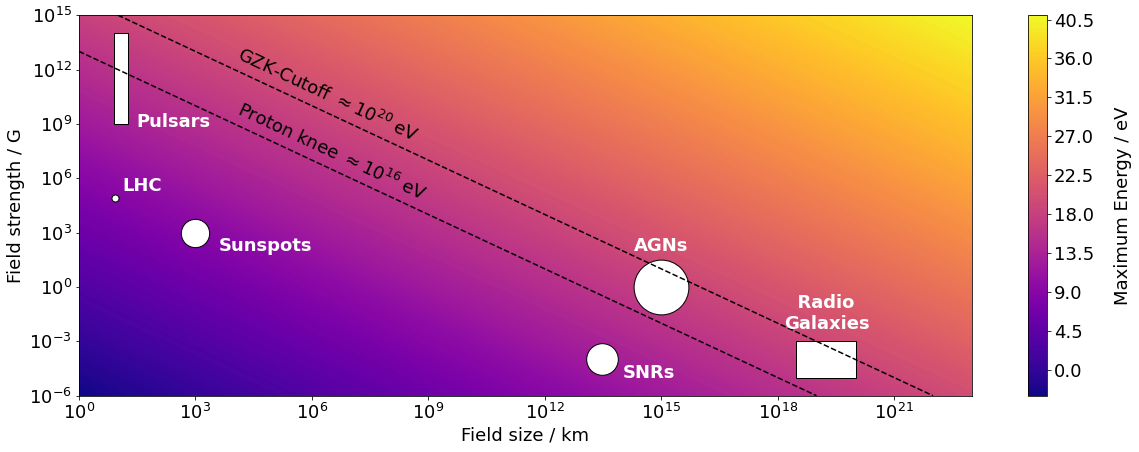
\includegraphics[width=1\textwidth]{./plots/hillas_plot.png}
	\caption{Rough estimate of field strength and size of different CR sources as well as the corresponding maximum energy estimated with 
    \autoref{eq:hillas-formula} ($\beta = Z = 1$). Isoenergetic lines mark notable points in the energy spectrum discussed in 
    \autoref{sec:cr-energy-spectrum}.}
	\label{fig:hillas-plot}
\end{figure}

\subsection{Propagation}
\label{ssec:cr-propagation}

Once a cosmic ray begins its journey from origin towards an eventual target, tracking its' trajectory is, ignoring external factors, in the literal sense, straight 
forward. 

For uncharged CRs ($\gamma$, $n$), the identification of a source is generally possible, as they travel mostly in a straight path. Possible interactions either 
demand the destruction of the particle (pair production, weak decay), or occur close to the source (e.g. Compton scattering), in which case the observed arrival 
direction will still be coincident with the actual source \cite{fermi201398}. Gravitational lensing effects in some cases alter the trajectory of extragalactic 
photons. Such phenomena (if present in the first place) are however well understood in the scope of general relativity, and can be corrected for 
\cite{bartelmann2010gravitational, bartelmann2001weak}.

Contrary, charged particles ($e^\pm$, $p$, ions) propagate along a non-trivial path due to deflections from solar- and galactic EM-fields. While the galactic field 
is coherent over large scales, numerous irregular magnetic domains, seeded in part by individual stars complicate CR propagation to essentially a three-dimensional 
random walk \cite{haverkorn2015magnetic}. It is thus challenging to pinpoint the origin of a charged cosmic ray. 

Nevertheless, related queries, such as for example the question whether or not a particle of given energy is likely to be of extragalactic origin can be answered by
examining the distribution of cosmic rays within a region of spacetime. The behaviour of a population of $n_i$ particles of type $i$ can be approximately recreated 
via the below transport equation:

\begin{equation*}
\label{eq:leaky-box-model}
\frac{\partial n_i}{\partial t} =   \underbrace{Q_i \vphantom{\left(\sum\limits_{j>i}\frac{p_{ij}}{\tau_{\text{spal.},\,j}} n_j\right)}}_\text{Source} 
 								  + \underbrace{\nabla D_i \left( \nabla n_i \right) \vphantom{\left(\sum\limits_{j>i}\frac{p_{ij}}{\tau_{\text{spal.},\,j}} n_j\right)}}_\text{Diffusion} 
								  - \underbrace{\frac{\partial k_i(E)}{\partial E} \vphantom{\left(\sum\limits_{j>i}\frac{p_{ij}}{\tau_{\text{spal.},\,j}} n_j\right)}}_\text{Energy} 
								  - \underbrace{\left( \frac{n_i}{\tau_{\text{spal.},\,i}} - \sum\limits_{j>i} \frac{n_j\,p_{ij}}{\tau_{\text{spal.},\,j}} \right)}_\text{Spallation}
								  - \underbrace{\left( \frac{n_i}{\tau_{\text{rad.},\,i}} - \sum\limits_{j>i} \frac{ n_j\,d_{ij}}{\tau_{\text{rad.},\,j}} \right)}_\text{Weak decay}
\end{equation*}

\begin{itemize}
	\item \textbf{Source} $Q_i$ :

	The source term is responsible for the creation of CR particles (of type $i$). The exact form of $Q_i$ will depend on the considered creation process. For 
	example, the near instantaneous creation of $n_\gamma$ photons in a \textbf{G}amma-\textbf{R}ay \textbf{B}urst (GRB) at time $t_0$ and location $\vec{r_0}$ can 
	be modelled like $Q_\gamma = n_\gamma \; \delta(\vec{r} - \vec{r_0})\delta(t - t_0)$.

	\item \textbf{Diffusion} $\nabla D_i \left( \nabla n_i \right)$ :

	The random walk mentioned above is accounted for in the diffusion term, which takes a similar form to the Stokes-Einstein equation. The diffusion 
	coefficient(s) $D_i$ in general take a tensor form due to anisotropic diffusion in different directions. Furthermore, $D_i$ is different for each particle 
	type, as the deflecting EM-fields couple to the respective charges $q_i$, which need not be equal in principle.

	\item \textbf{Energy loss} $\partial k_i(E)\,/\,\partial E$ :

	During propagation, a cosmic ray can interact with the ISM, and lose energy in the process. If this happens often enough, the CR is eventually thermalized and 
	does not contribute to the population any longer. Different interaction channels for different CR types $i$ require different loss models $k_i(E)$ for each 
	type. 

	\item \textbf{Spallation} $\left( n_i\,/\,\tau_{\text{spal.},\,i} - \sum n_j\,p_{ij}\,/\,\tau_{\text{spal.},\,j} \right)$ :

	Nuclear spallation describes the process of violent disintegration of a target nucleus upon being struck by an energetic projectile. The resulting fragments
	can retain energies up to the projectiles energy. The spallation term in the transport equation considers both the destruction (first term), as well as 
	creation (second term) of CRs $i$ from heavier types $j$. It is assumed that spallation from type $j \rightarrow i$ occurs at a constant probability of 
	$p_{ij}$ in a characteristic time frame $\tau_{\text{spal.},\,j}$.

	\item \textbf{Weak decay} $\left( n_i\,/\,\tau_{\text{rad.},\,i} - \sum n_j\,d_{ij}\,/\,\tau_{\text{rad.},\,j} \right)$ :

	If a particle $j$ is weakly unstable ($\tau_{\text{rad.},\,i} < \infty$) there is a nonzero chance $d_{ij}$ it decays into a daughter nuclei of some type $i$ 
	during propagation. The decay term reflects this and describes both decay from heavier and decay into lighter nuclei.
\end{itemize}

TODO: Simulation?

\subsection{Composition}
\label{ssec:cr-composition}

\begin{figure}
	\centering
	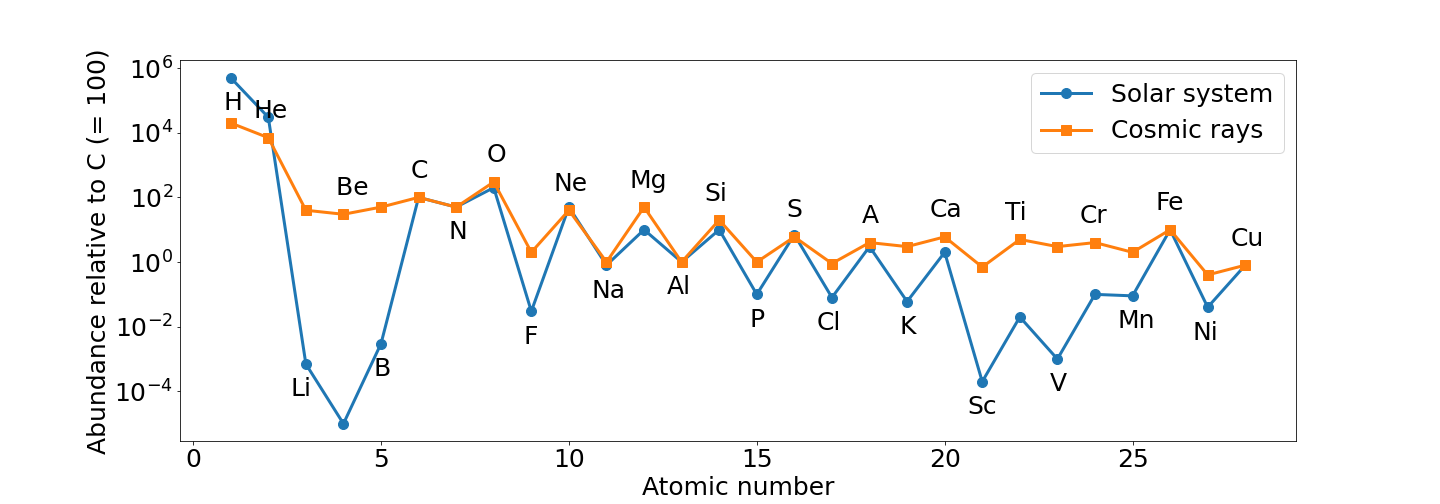
\includegraphics[width=1\textwidth]{./plots/cosmic_ray_composition.png}
	\caption{}
	\label{fig:cr-composition}
\end{figure}

\section{Energy spectrum}
\label{sec:cr-energy-spectrum}



\section{Extensive air showers}
\label{sec:extensive-air-showers}